% TODO maybe introduce weaks and softs??

\chapter{Memory Fundamentals}

Before getting into the details of how to implement your lifetime requirements,
it is important to understand some of what the fundamentals of memory management
in languages like Java. The Java language has a \emph{managed runtime}. In part,
this means that, as a Java program runs, a runtime environment assumes the burden
of key aspects of memory management. This level of management includes as
automatic garbage collection of both instances and Java classes. Therefore, Java
has feature that govern, on your behalf, important aspects of the lifetime of
objects. You need to appreciate what the runtime is doing for you, before
considering how to reshape object lifetimes to better suit your needs.

Designing a lifetime management strategy requires that you take the tools that
Java provides, and combine them with other strategies implemented on top of Java.
The built-in mechanisms handle some aspects of the common patterns of object
lifetime. Unfortunately, they often appear in the form of low-level JVM hooks,
and so require careful coding to make correct use of them.

This chapter introduces the basics of the garbage collector, and how the Java
managed runtime governs object lifetimes. Then, it walks you through the
lifecycle of typical objects from allocation to eventual garbage collection. If
you are comfortable with the basics of memory management, you may discover that
you can skip to the next chapter.

\section{The Garbage Collector}
The \jre decides when the storage allocated to an object should be reclaimed.
This decision is based on a number of criteria. The point of reclamation
depends on the settings you have chosen for various policy knobs, and is also
affected by choices you have made in the application code. However, in most
cases, there is a common structure to the schedule of when objects are
collected.

\paragraph{The Collection Schedule}
Most contemporary garbage collectors deallocate storage in a series of bulk
steps. In almost all \jres, memory is not reclaimed one object at a time.
Instead, to amortize the costs involved in reclamation, the garbage collector
often lets reclaimable objects pile up for a while. It then collects then en
masse. As objects are allocated, memory consumption can be observed to increase,
up until some maximum allowed amount. At this point, the collector reclaims
unused memory, and the process starts again. In this way, memory consumption over
time often assumes a sawtooth edge, such as those shown in
\autoref{fig:timeline-base-session-temps-with-cache}.
\index{Sawtooth Pattern}

\paragraph{Configuration Settings}
You can guide the frequency of collection, which will change the slope of this
sawtooth curve to be either more or less jagged. In one common case, the garbage
collector will wait until all available memory is consumed before reclaiming
storage.  In Java, you can configure this ceiling by supplying a sizing to the
\code{-Xms} (initial ceiling) and
\code{-Xmx} (maximum ceiling) command line options. \index{-Xms command line setting}
\index{-Xmx command line setting} The \jre will begin with a ceiling at the
former level. If collections are occuring too frequently, the \jre may decide to
increase the \emph{current} ceiling to a higher level. As the need for memory
fluctuates, so the \jre will raise or lower the current ceiling level. The
current ceiling will always be some value lower than the maximum, \code{-Xmx},
setting. One such scenario, of increasing ceiling level, is illustrated in
\autoref{fig:timeline-base-session-temps-with-leak}.


\paragraph{What a Collection Collects}

\paragraph{The Nursery, Permspace, and Constant Pools}
\index{Nursery}
\index{Permspace}

\paragraph{Finalization and Phantom Referenes}
\index{Finalization of objects}
\index{Phantom References}

\paragraph{Class Unloading and Lifetime of Statics}

A \code{static} field of an object is one way that Java gives you to indicate
that you want an object to live forever.
\index{Class Unloading}
\index{Static fields}

\paragraph{Concurrent, Parallel, and Real-time Collection}
\index{Concurrent GC}
\index{Parallel GC}
\index{Real-time GC}


\section{The Object Lifecycle}
%Every object created by your application lives for an interval of time from its
%creation to the point that the Java runtime gets around to collecting it. An object's {\em natural} lifetime is defined by the
%interval of time between its first and last necessary use. %cite drag paper
%here?


In a \emph{well-behaved} application, an object's lifetime spans its allocation,
use, and the short period during which the \jre takes control and reclaims the
space. For some subset of an object's actual lifetime, that is the time from
creation to reclamation, your application will make use of the data stored in its
fields. \autoref{fig:typical-lifecycle} illustrates the lifecycle of a typical
object in a well behaved application.

\begin{figure}
	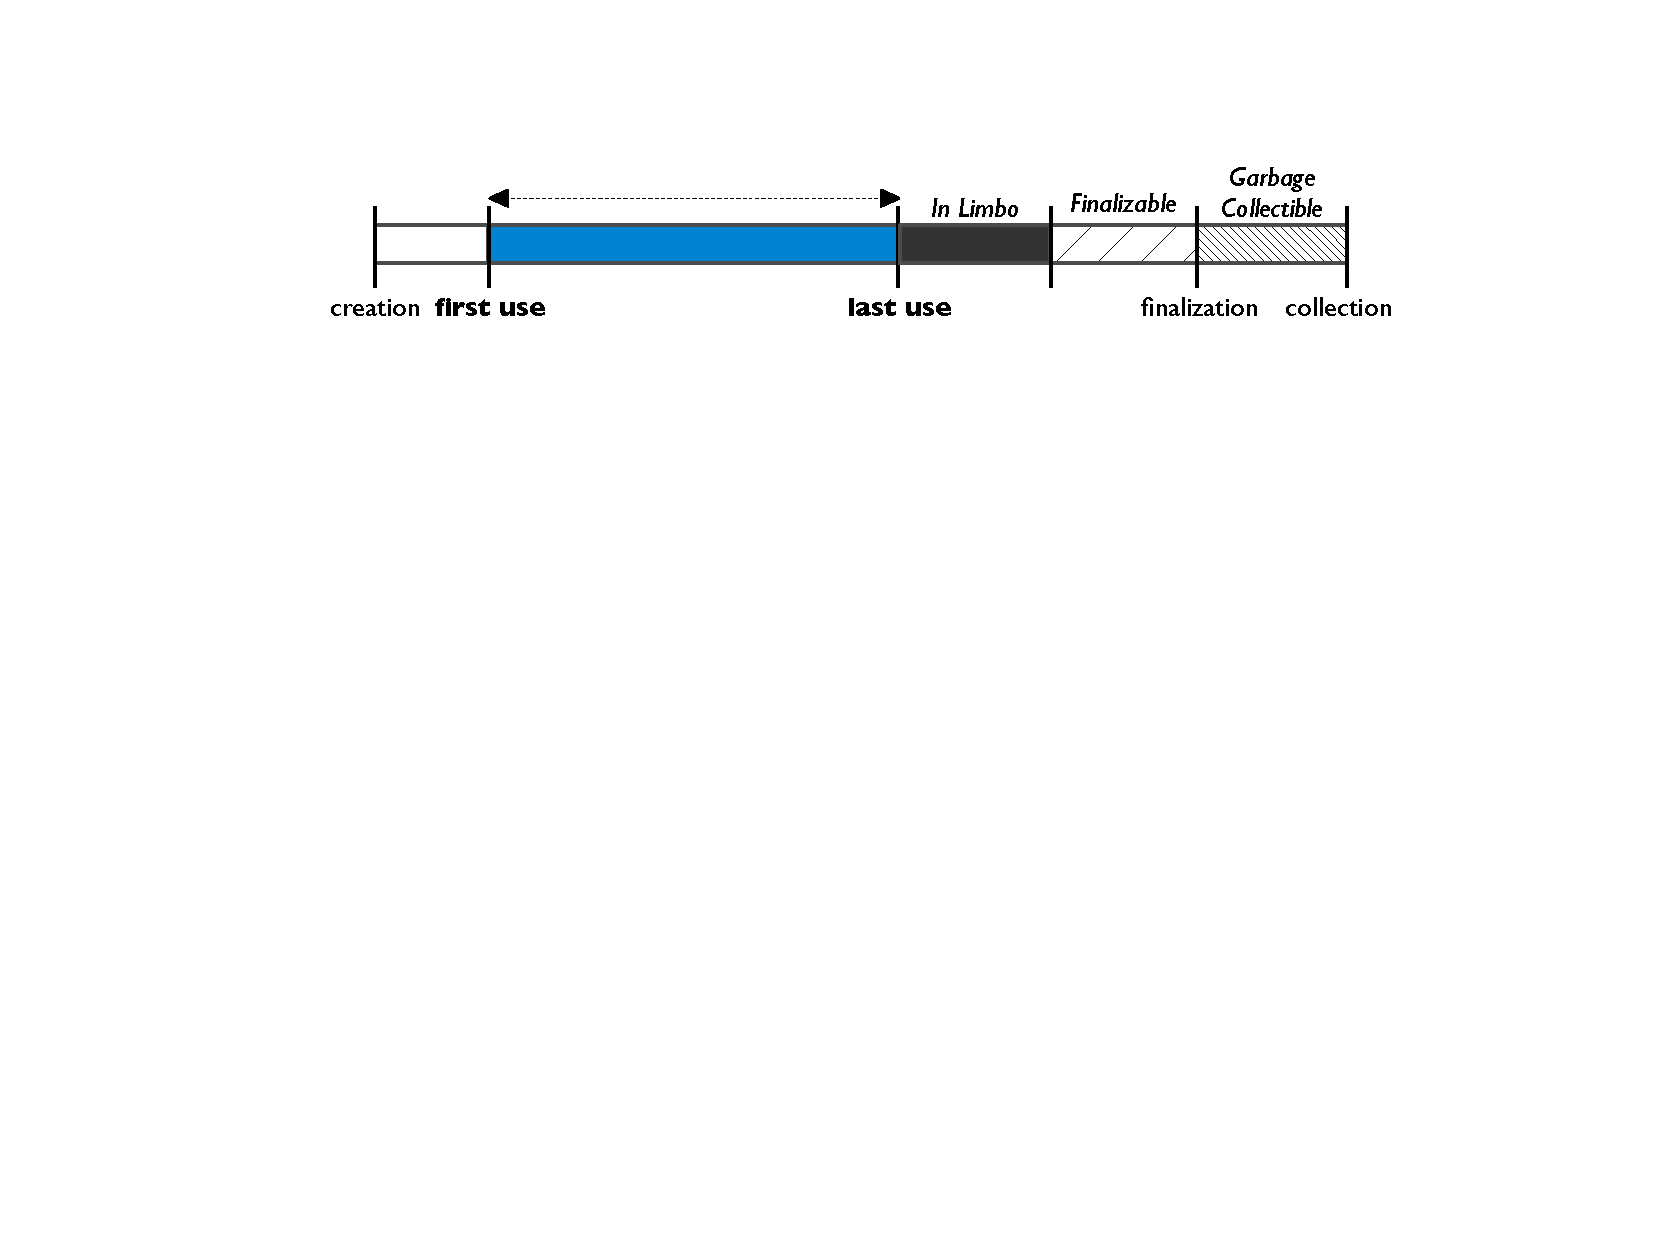
\includegraphics[width=0.9\textwidth]{part4/Figures/lifetime/object-lifecycle}
	\caption{Timeline of the life of an object.}
	\label{fig:typical-lifecycle}
\end{figure}

\begin{example}{Parsing a Date} Consider a loop that shows an easy way to parse
a list of dates. What objects are created, and what are their lifetimes?
\begin{shortlisting}
for (String string : inputList) {
	ParsePosition pos = new ParsePosition(0);
	SimpleDateFormat parser = new SimpleDateFormat();
	System.out.println(parser.parse(string, pos));
}
\end{shortlisting}
\end{example}

For each iteration of this loop, this code takes a date that is represented as a
string and produces a standard Java \class{Date} object. In doing so, a number of
objects are created. Two of these are easy to see, in the two \code{new} calls
that create the parse position and date parser objects. The programmer who wrote
this created two objects, but many more are created by the standard libraries to
finish the task. These include a calendar object, number of arrays, and the
\class{Date} itself. None of these objects are used beyond the iteration of the
loop in which they were created. Within one iteration, they are created, almost
immediately used, and then enter a state of \emph{limbo}.

\callout{limbo}{Objects in Limbo}{
\index{Limbo}
In limbo, an object will never be used again, or at least not for long time,
but the \jre doesn't yet know that this is the case. The object hangs
around, taking up space in the Java heap until the point when it exits limbo.}

The \code{pos} object represents to the parser the position within the
input string to begin parsing. The implementation of the \code{parse} method
uses it early on in the process of parsing. Despite being unused for the
remainder of the parsing, the \jre does not know this until the current
iteration of the loop has finished. This time in limbo also includes the
entirety of the call to \code{System.out.println}, an operation entirely
unrelated to the creation or use of the parse position object. Once the current
loop iteration finishes, these two objects will exit limbo, and become garbage
collectible.\index{Exiting Limbo}

\begin{figure}
	\centering
	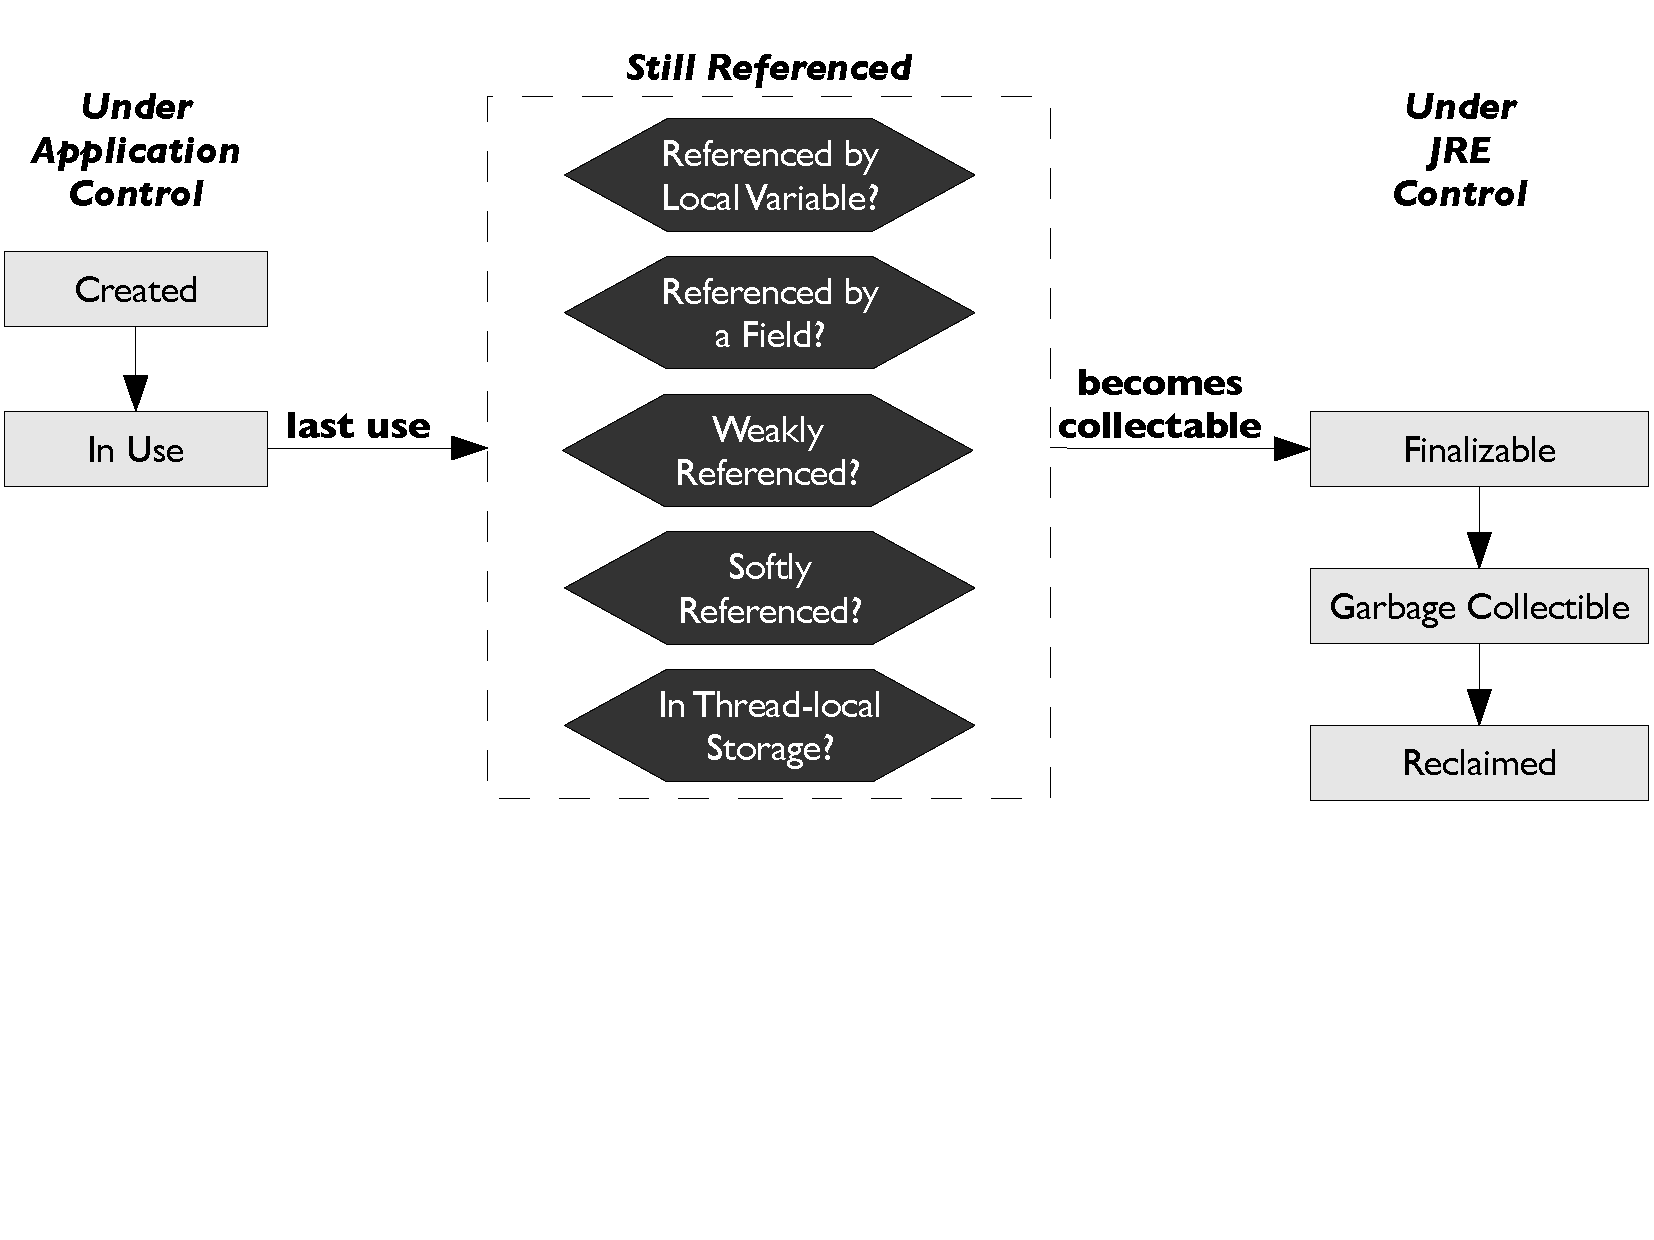
\includegraphics[width=\textwidth]{part4/Figures/lifetime/states}
	\caption{After its last use, an object enters a kind of limbo: the application
	is done with it, but the \jre hasn't yet inferred this to be the case. When an
	object exits limbo depends on the way it is referenced.}
		\label{fig:limbo-exit}
\end{figure}


\begin{comment}
\begin{figure}
	\centering
	\subfigure[The lifecycle of a typical object and its data.]{
	\label{fig:typical-lifecycle1}
			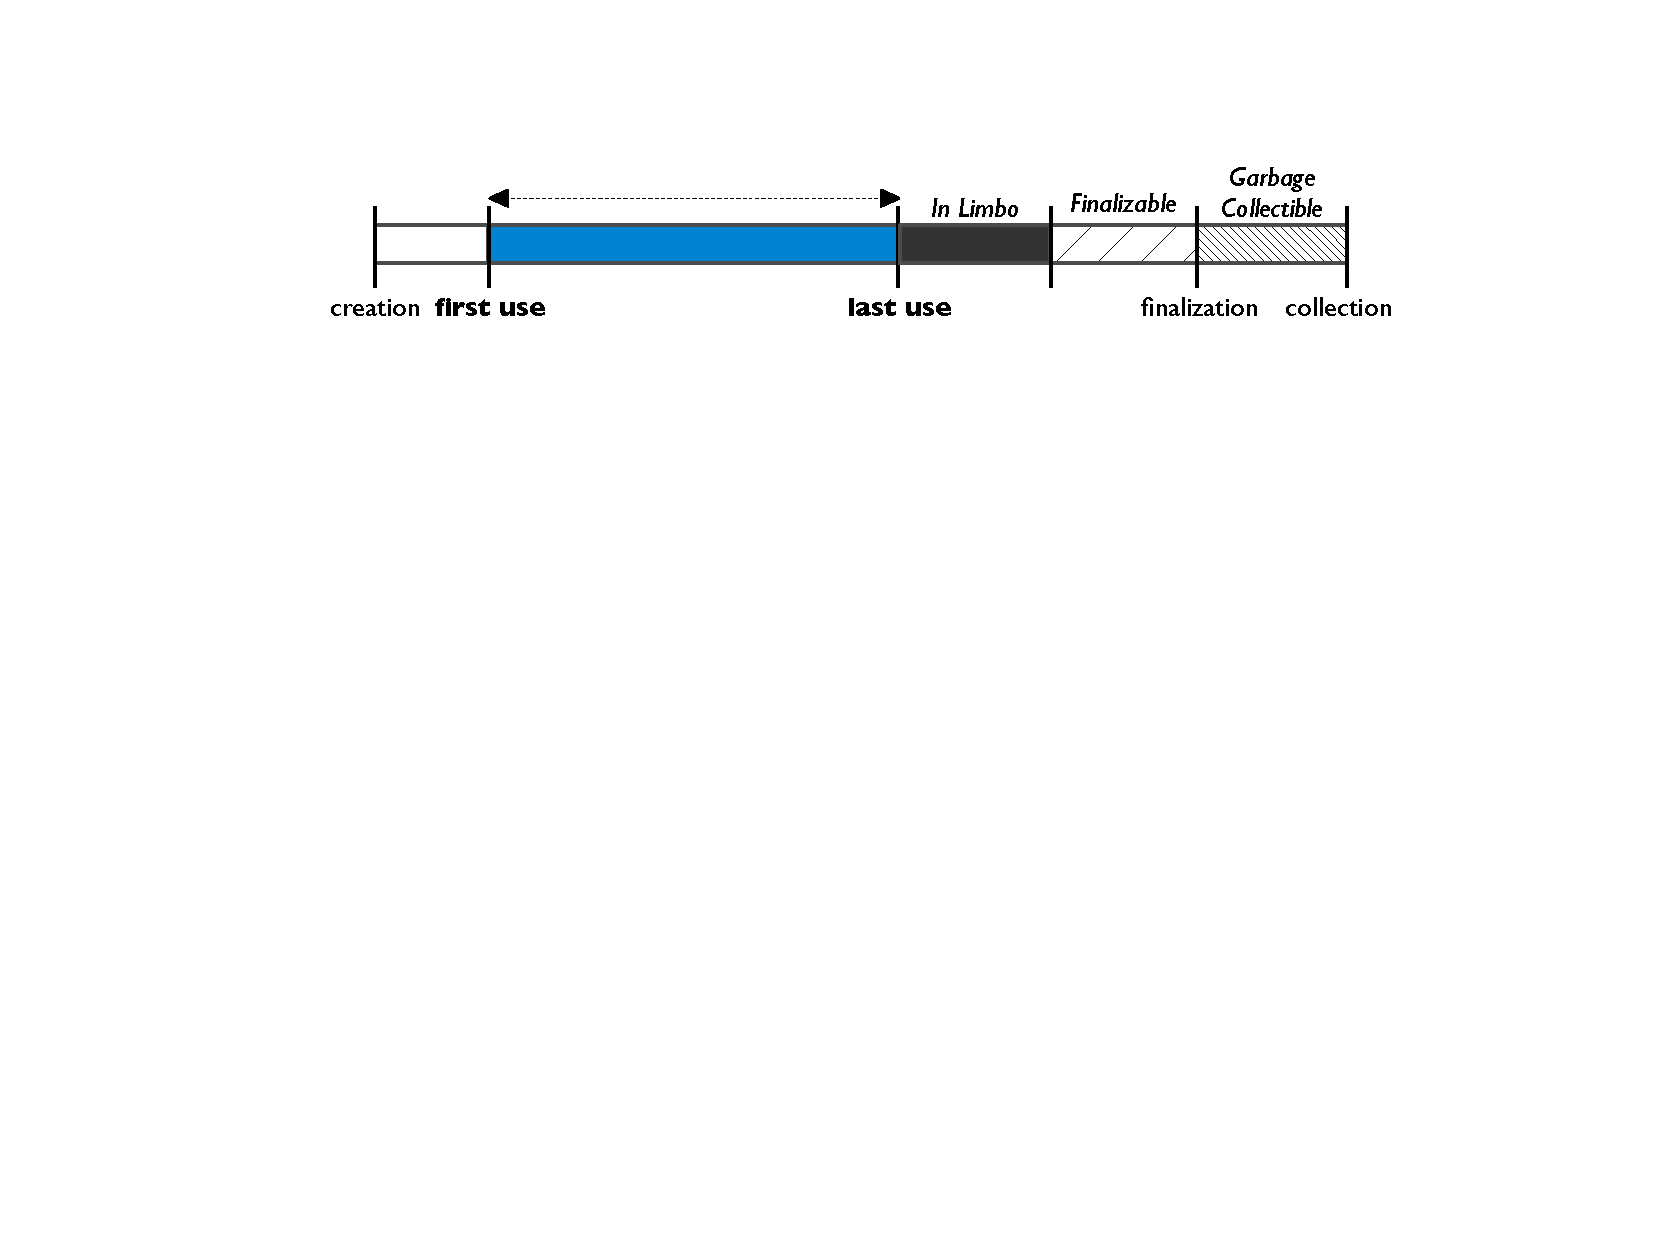
\includegraphics[width=0.95\textwidth]{part4/Figures/lifetime/object-lifecycle}
	}
	\subfigure[A situation where there are long periods between uses of an
	object's data.]{
	\label{fig:typical-lifecycle2}
		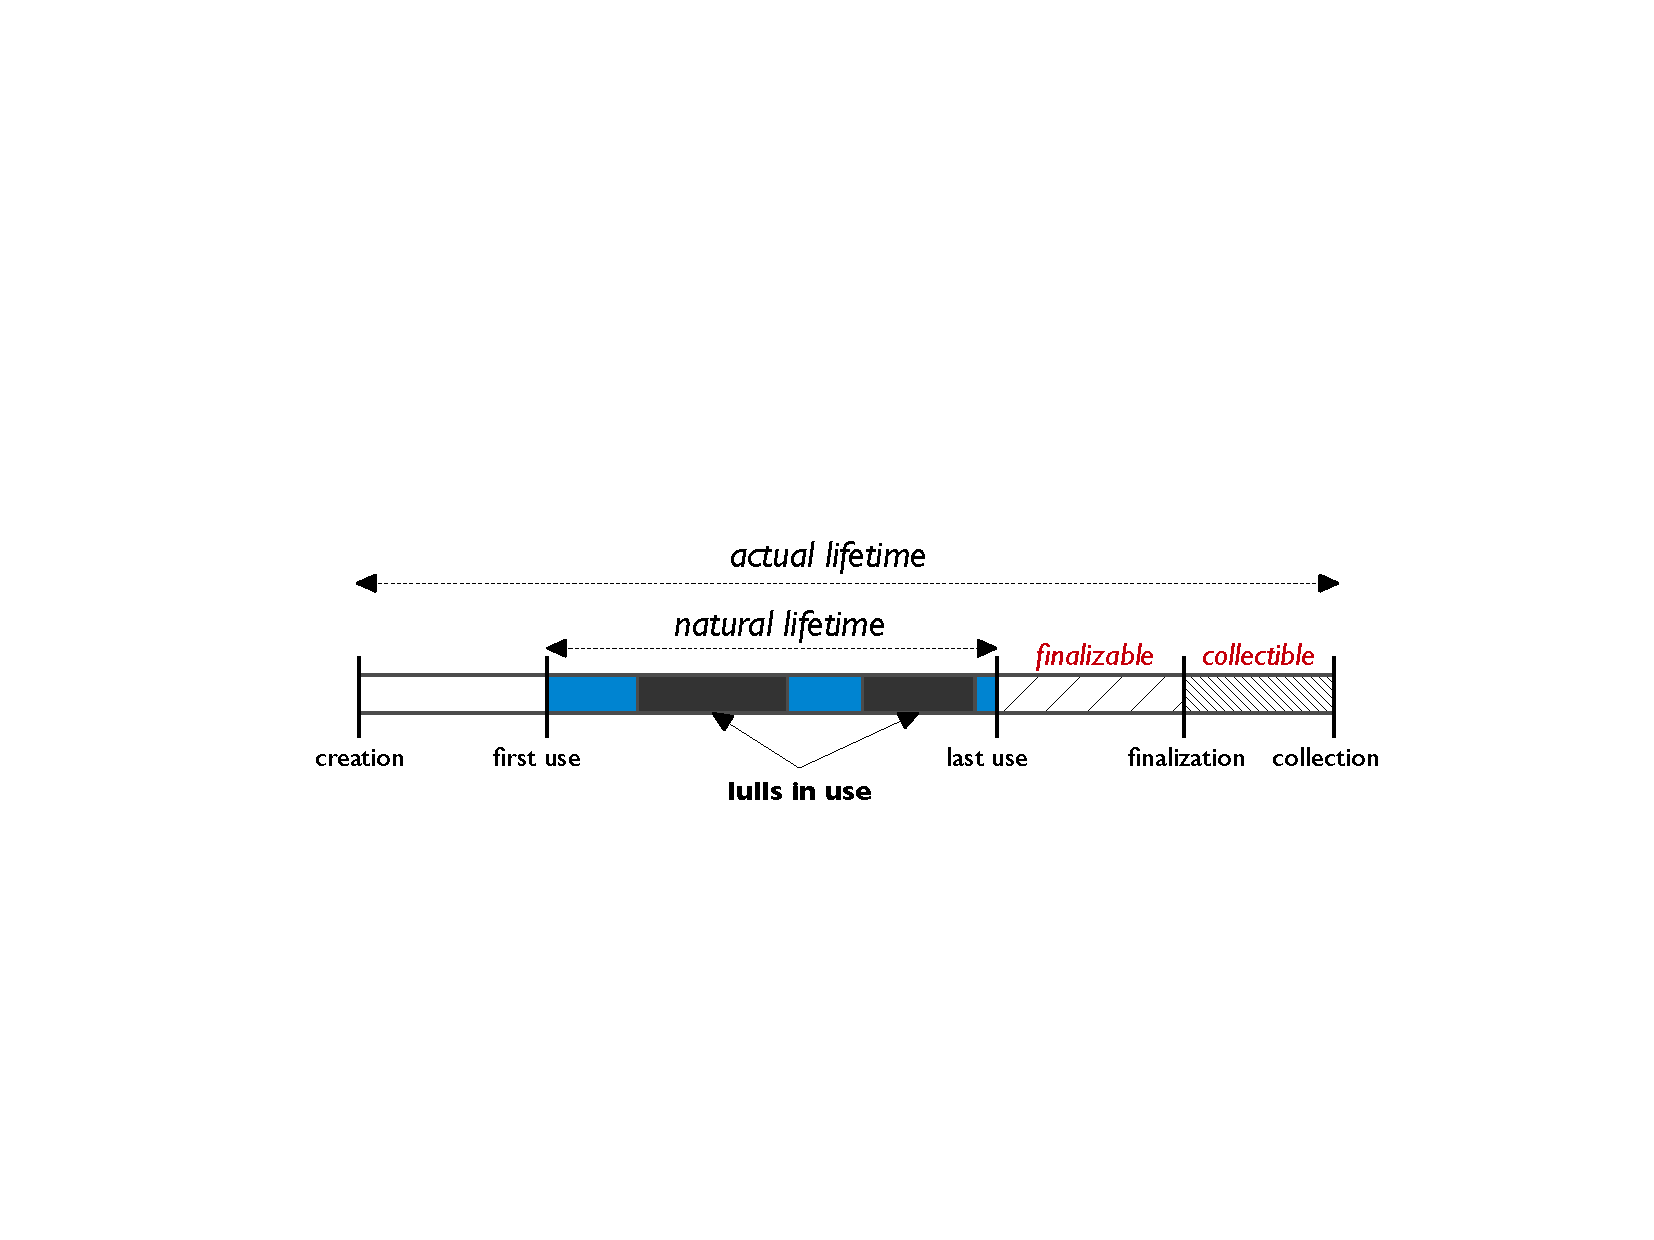
\includegraphics[width=0.95\textwidth]{part4/Figures/lifetime/object-lifecycle-lulls}
	}
	\subfigure[The lifecycle of the data  that is loaded from
	disk three times, and the objects that store it.]{
	\label{fig:typical-lifecycle3}
		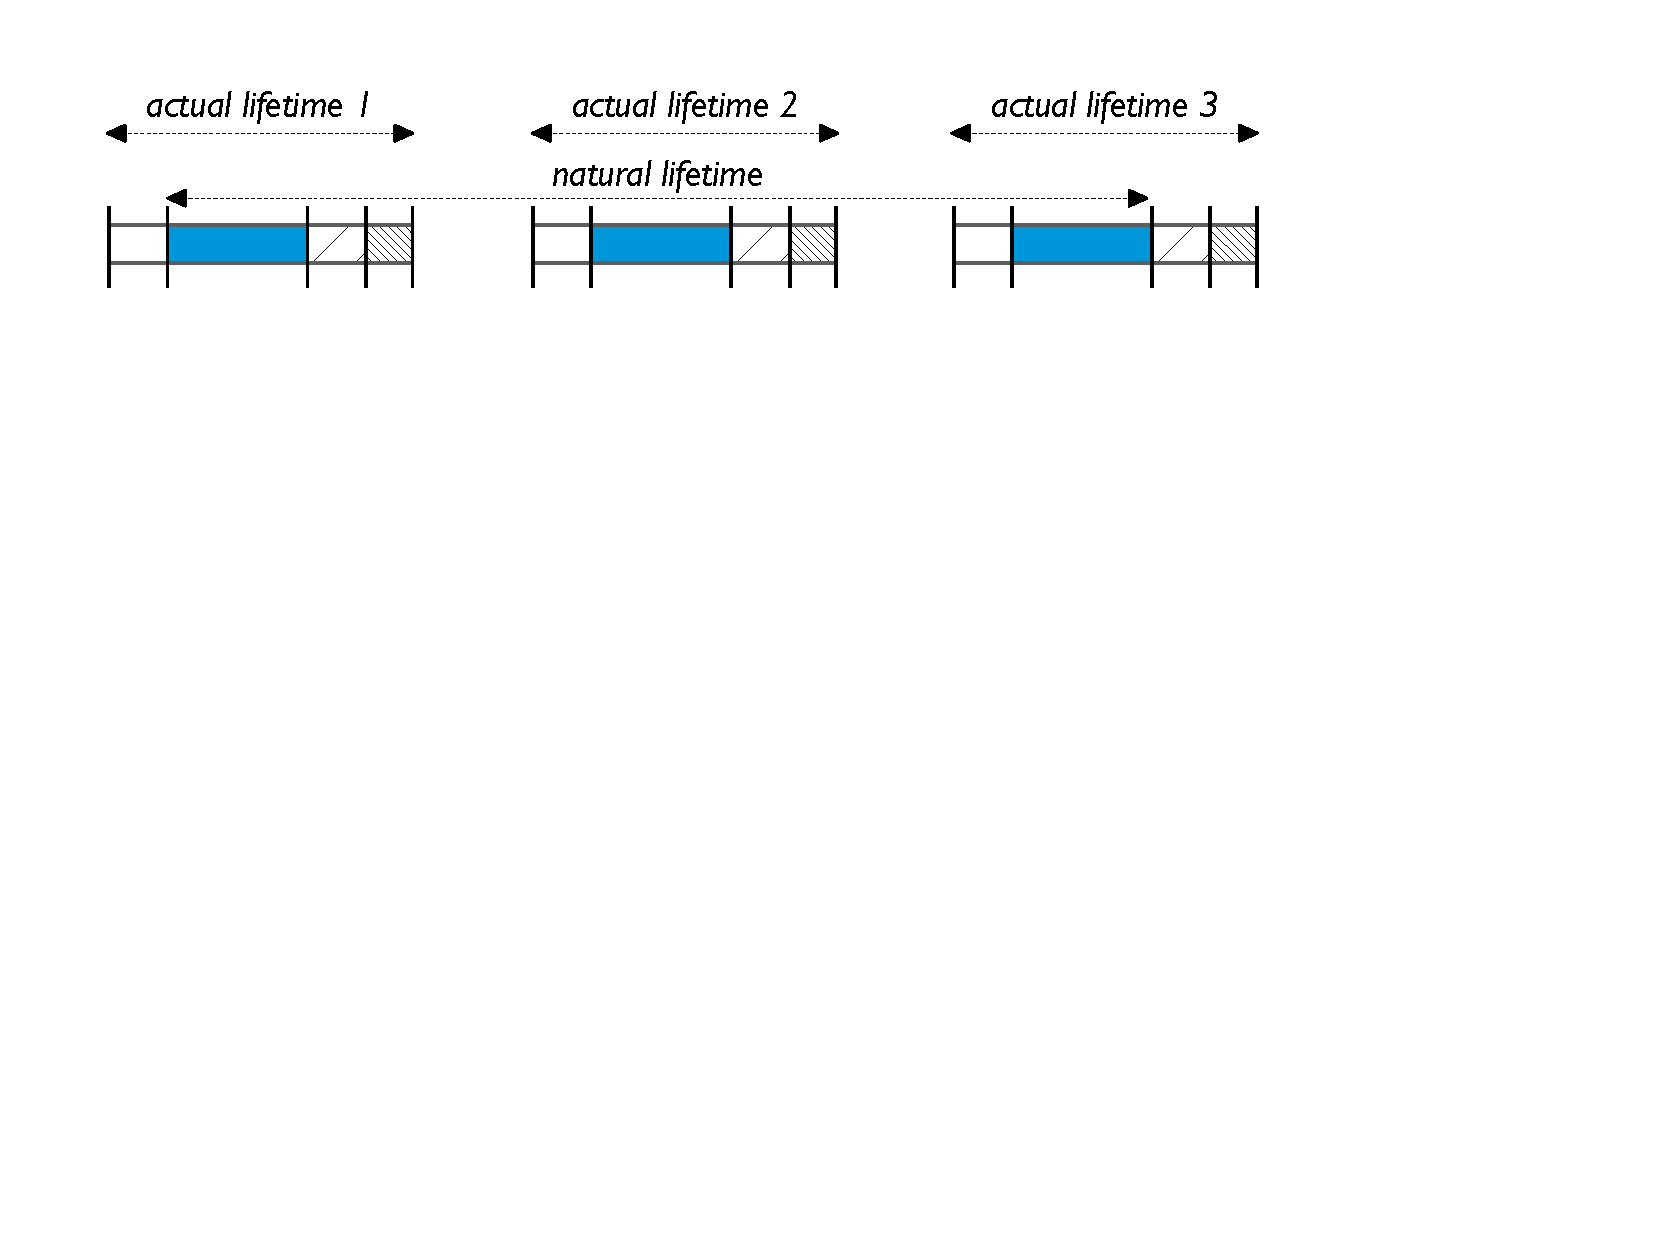
\includegraphics[width=0.9\textwidth]{part4/Figures/object-lifecycle2}
	}
	\caption{Examples of Natural and Actual lifetimes.}
	\label{fig:typical-lifecycle}
\end{figure}
\end{comment}


\section{Basic Management Mechanisms}
DO WE NEED THIS?

The point at which an object exits its limbo depends upon how it is referenced by
other objects. One can always assure that an object exits limbo by modifying your
code to overwrite all references to that variable. If an object is no longer
referenced at all, then it will exit limbo immediately.\footnote{Talk about
reference cycles?} For example, a common way to do this is by assigning
references to the value \code{null}. This is tricky in many cases, because it may not be easy to
know where all those references emanate from. Who is to say that, when one calls
the \code{parse} method of a \class{SimpleDateFormat} object, that it does not
squirrel away a reference to the \class{ParsePosition} passed as a parameter? The
API contract for \code{parse} makes no such claims, one way or the other. This is
certainly calls to mind the worst of the days of explicitly managing memory in a
language like C.


Still, one can't always rely on automatic mechanisms to guide an object out of
limbo in a timely fashion.
\autoref{fig:limbo-exit} and \autoref{tab:limbo-exit}
illustrate how an object may exit limbo. 
A garbage collector only knows that an object is ready to
be collected based on {\em reachability}: how the objects point to eachother.
If, as in the \class{ParsePosition}
or \class{SimpleDateFormat} objects from our example, the object is referenced
only by a local variable of a method, the \jre will not consider reclaming its
storage until the variable's scope exits; e.g. when the loop continues to the
next iteration, or when the method returns, depending on the scope of the
variable that references the object. If the object is referenced only by a
field of another object, then it must wait for that other object to exit limbo
before it can do so. 
An objects pointed to be only by a static field has a good chance of never
being collected. A class only exits limbo when it is unloaded by the \jres
class loading mechanism, which is unlikely to happen if it has static fields
that reference other objects. Therefore, unless that field is overwritten,
objects pointed to by static fields are likely never to exit limbo.